\documentclass[french,12pt,notitlepage]{report}
\usepackage[utf8]{inputenc}
\usepackage[T1]{fontenc}
\usepackage{lmodern}
\usepackage[a4paper]{geometry}
\usepackage[francais]{babel}
\usepackage{graphicx}


\begin{document}
	\title{Functional data analysis applied to neurology}
	\author{Clément Bonvoisin, Pierre Ludmann}
	\date{30 juin 2014}
	\maketitle

	\begin{abstract}
  
Il s'agit de segmenter des signaux de marche,
dans le cadre d'une collaboration du CMLA (ENS Cachan) et Cognac-G (Paris V).
%Quels sont les travaux déjà accomplis dans ce domaine dans le monde?

On propose donc ici des algorithmes pour détecter des ruptures.
Cela permet en aval aux médecins de mieux étudier les différentes régimes de marche.
Un algorithme efficace et rapide semble encore manquer.

Si la détection d'un unique changement trouve des implémentations reconnues,
on a cherché à généraliser à de multiples ruptures.
Aussi on a changé le paramètre de décision : on exige un nombre précis de résultats plutôt qu'un seuil de détection.

Malgré de fortes hypothèses de travail,
on obtient des résultats statisfaisants sur des signaux réels et synthétiques
bien que des améliorations restes possibles.

Son utilisation doit faire place à un apprentissage sur les segments de régime obtenus.
	
	\end{abstract}

	\tableofcontents

	\chapter{Introduction au problème}
	\section{Motivations}
		La motivation initiale de ce stage provient de la médecine, et plus particulièrement de la neurologie. Le projet, piloté par le groupe Cognac-G, vise à analyser en détail des signaux physiologiques, issus d'une expérience très simple.
	\\ \\
	Le protocole expérimental se décline comme suit :
	\begin{itemize}
		\item On place sur le patient un ensemble de capteurs : un à la tête, un à la ceinture, et un sur chaque pied. Ces capteurs sont des centrales inertielles, qui permettent une mesure de l'accélération et de la vitesse angulaire du patient.
		\item On lance l'acquisition. Pendant quelques secondes, le patient est à l'arrêt. Puis, il commence à marcher sur une dizaine de mètres, effectue un demi-tour, et fait une marche retour. Il s'arrête, et on peut alors arrêter l'acquisition.
		\item On replace alors les signaux obtenus dans un repère adapté au corps humain, formé de trois axes : l'axe antéro-postérieur, l'axe transversal (aussi appelé médio-latéral), et l'axe longitudinal (aussi appelé axe vertical).
	\end{itemize}
	
	\begin{figure}[!h]
		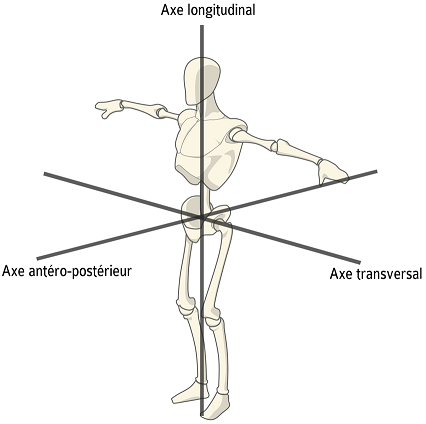
\includegraphics[scale=0.3]{axis.png}
		\caption{Le repère (antéro-postérieur; médio-latéral; vertical)}
		\label{axis}
	\end{figure}
		
	\vspace{1pc}
	
	On obtient alors des signaux physiologiques ayant 6 composantes distinctes pour chaque capteur, à une fréquence d'acquisition dépendante de la centrale inertielle utilisée ; actuellement, le projet Cognac-G dispose d'instruments permettant un échantillonnage à 100Hz.
	
	\begin{figure}[!h]
		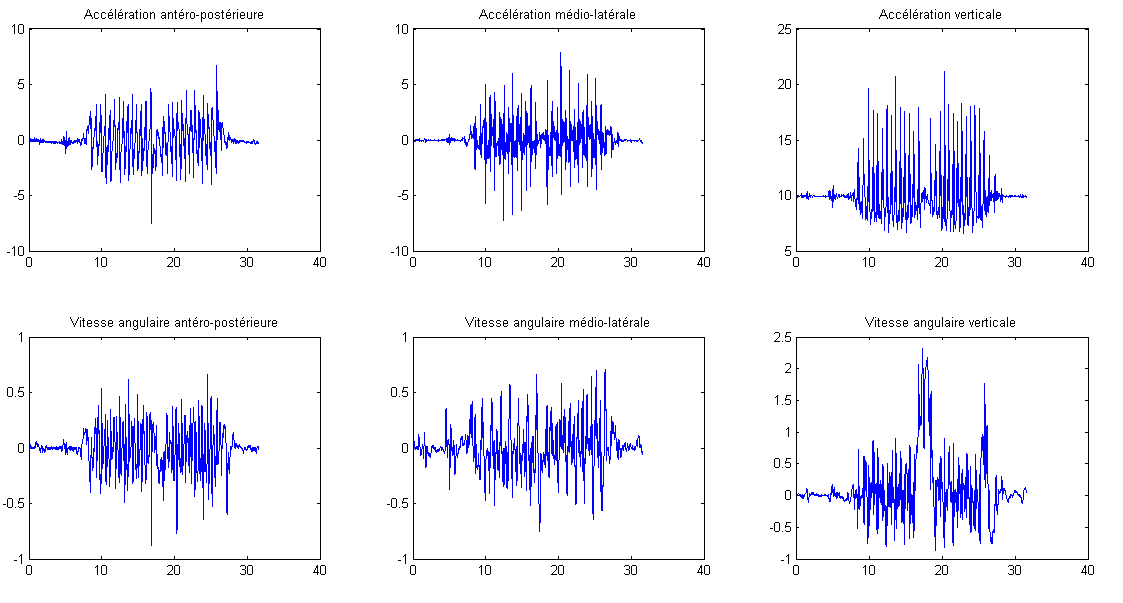
\includegraphics[scale=0.5]{ex_signal_back.png}
		\caption{Un exemple de signal de marche (enregistré à la ceinture)}
		\label{ex_signal_back}
	\end{figure}
	
	Sur ces signaux apparaissent de manière claire les différentes phases de l'expérience :
	\begin{itemize}
		\item Dans un premier temps, le patient est à l'arrêt, les 6 signaux sont quasiment constants (on n'observe que du bruit)
		\item Dans une seconde phase, le patient commence à marcher : on observe une phase transitoire entre l'arrêt et la marche dite de croisière
		\item La troisième phase de l'expérience correspond à la marche de croisière : le patient effectue une dizaine de mètres
		\item On observe ensuite le demi-tour (particulièrement sur les composantes verticales du signal), qui dure environ 1 seconde
		\item Puis, on a une nouvelle phase de marche, retour cette fois-ci
		\item Finalement, le patient s'arrête : on a à nouveau une phase transitoire, puis l'arrêt total du patient (où il ne reste plus que du bruit)
	\end{itemize}
	
	\vspace{1pc}
	
	Partant de ces constatations, on peut donc constater que les signaux acquis par les centrales inertielles peuvent être segmentés, qu'on peut isoler les différentes phases de l'expérience. Sur un signal, cela peut être fait de manière manuelle ; néanmoins, pour un neurologue enregistrant de manière régulière ce type d'expérience, il est concevable de désirer des algorithmes robustes permettant de traiter de manière automatique le problème de la détection des points de changement, décomposant ainsi le signal en sous-signaux correspondant à chacune des phases de l'expérience, afin de pouvoir les analyser séparément.
	
	\section{Formalisme mathématique}
	Afin de pouvoir traiter mathématiquement le problème, il nous faut tout d'abord poser des définitions claires sur l'objet du problème : il s'agit donc de définir ce qu'est une rupture, au sens mathématique.
	\\ \\
	La littérature propose une approche statistique du problème : on considère les signaux comme la réalisation d'une suite (finie) de variables aléatoires :
%Proposer ici des références bibliographiques...
	\begin{equation}
		(x_i)_{i \in \{1..N\}} = (X_i(\omega))_{i \in \{1..N\}}
		\label{11}
	\end{equation}
	
	Ce formalisme, qui peut paraître quelque peu abstrait en première approche, permet d'exprimer de manière simple la notion de rupture dans un signal.
	\\ \\
	Sur les signaux précédents, on constate, par exemple, une différence nette d'écart-type entre la phase à l'arrêt et la phase de marche ; de même, sur la vitesse angulaire verticale, on constate un changement de moyenne entre les phases de marche et le demi-tour. Il paraît donc naturel de considérer la distribution statistique des différents points d'un signal multivarié pour formaliser le concept de rupture.
	\\ \\
	On comprend alors la définition donnée par la littérature d'un point de rupture à un instant $t_0$ :
	\begin{equation}
	\begin{array}{ll}
			\forall t \in [1, t_0-1], X_i \sim p_0 \\
			 \forall t \in [t_0, N], X_i \sim p_1 \\
	\end{array}
	\end{equation}
	
	On généralise de manière évidente au cas de $n$ ruptures aux points $(t_i)_{i \in \{0, n-1\}}$ :
	
	\begin{equation}
	\begin{array}{lll}
		\forall i \in \{0, n-1\}, \\
		\forall t \in \{t_{i-1}, t_i-1\}, X_i \sim p_{i-1} \\
		\forall t \in \{t_i, t_{i+1}-1\}, X_i \sim p_i
	\end{array}
	\end{equation}
	Où l'on a posé : $t_{-1} = 1$ et $t_n = N$.
	\\ \\
	Ce problème étant formalisé, il s'agit maintenant de trouver des méthodes pour détecter ces points de rupture.
	
	\chapter{Algorithme CUSUM : résolution du cas d'une seule rupture}
	
	\chapter{Cas de plusieurs ruptures : implémentation dichotomique}
	
	\chapter{Cas de plusieurs ruptures : implémentation par fenêtres}
	
	\chapter{Évaluation des performances}
	
	\chapter{Conclusion}
\end{document}
